\documentclass[a4paper,11pt,twoside]{report}
\usepackage[utf8]{inputenc}
\usepackage[top=2.5cm,bottom=2.5cm,outer=2.5cm,inner=2.0cm]{geometry}

\usepackage{amssymb}
\usepackage{amsmath}
\usepackage{booktabs}
\usepackage{hyperref}
\usepackage[noabbrev,capitalise]{cleveref}
\usepackage{colortbl}
\usepackage{color,soul}
\usepackage{xcolor}

\usepackage{enumitem}
% \setlist[enumerate,1]{label=\color{blue}(\arabic*)}
\setlist[enumerate,1]{label=(\arabic*)}

\usepackage{graphicx}
\usepackage{helvet}
\renewcommand{\familydefault}{\sfdefault}

\usepackage{hyperref}
\hypersetup{
	colorlinks = true,
	linkbordercolor = {white},
}

\usepackage{listings}

\usepackage{setspace}
\renewcommand{\baselinestretch}{1.3}

\usepackage{siunitx}
\usepackage{threeparttable}
\usepackage{multirow}

\begin{document}

\begin{center}
	{\large\textbf{Imaging Neuroscience \#203: Responses to Editors and Reviewers}}
\end{center}

% Robin: cortex / brain stem / hippocampus /

% ========================================
%     Editor
% ========================================


% ========================================
%     Reviewer 1
% ========================================

\noindent \underline{\textbf{Reviewer \#248}}

\textit{Authors have partially addressed my previous comments. A list of pending issues is listed below:}

\vspace{1em}

\noindent \textit{Major:}

\begin{enumerate}
    \item [1)] \textit{The experiment is generally satisfactory, but its description is a bit confusing (especially point b) below:
        \begin{enumerate}
            \item [a)] L125: "Protocol \#1 with six-shot iEPI and without in-plane undersampling was implemented" then (L131) "We then retrospectively reduced the four-shot data to only one shot", guess there is a misprint in L125 which should be four-shot rather than six-shot?
            \item [b)] L132: "with the proposed $k_y$ shifting to simulate three-fold in-plane undersampling" $\rightarrow$ as there is no in-plane undersampling in Protocol \#1 in the baseline data (according to Table 1) this sounds a bit confusing, if 1 out of 4 shots are used this would be four-fold in-plane undersampling, so unclear how you reach three-fold in-plane undersampling? Guess you mean something like "three-fold in-plane interleaving"? A few more details may help here.
            \item [c)] L133: "JETS reconstruction was performed on all data" $\rightarrow$ "all data" is a bit vague, please reword.
        \end{enumerate}}

    \begin{enumerate}{\color{blue}
        \item [a)]Sorry about the misprint. We corrected it as four-shot.
        \item [b)] Thank you for the question.
        You are right that "1 out of 4 shots are used",
        so it is four-fold in-plane undersampling.
        We corrected this in the manuscript.
        \item [c)] Thank you. This sentence has been reworded.}
    \end{enumerate}

    \item [2)] \textit{Fine, only a small detail, L61: "acquisition. SPA-LLR" $\rightarrow$ "acquisition and SPA-LLR"}

    \hspace{1em} {\color{blue} Done.}

    \item [3)] \textit{There are some pending issues:
        \begin{enumerate}
            \item [a)] Authors could drop a line in text indicating why they use JULEPS rather than MUSSELS.
            \item [b)] Results of MUSE $+$ Denoiser look stronger than with previous denoiser. Indeed, now they are quite comparable to JETS (bit noisier but also bit sharper). A question is whether complex denoiser is applied before (replacing TV) or after shot-combination of MUSE? May make sense to try both approaches. Also, authors may want to draw a few lines about potential synergies between their LLR and the denoiser.
            \item [c)] In previous version you also included comparisons for FA and different b-values but these seem missing here. I think that maintaining comparisons at different b-vals could be particularly useful.
        \end{enumerate}}

    \begin{enumerate} {\color{blue}
        \item [a)] Done.
        \item [b)] The complex denoiser is applied after
        the shot combination in MUSE.
        The local-PCA denoiser operates on spatial-diffusion matrices,
        whereas MUSE reconstructs one DWI at a time.
        Therefore, the denoiser is only applicable
        after the reconstruction of all DWIs,
        and is not possible before the completion of MUSE
        (e.g.~before shot combination). \\
        We added "potential synergies between their LLR and the denoiser"
        into Discussion.
        \item [c)] We added back the three-shell data.}
    \end{enumerate}

    \item [4)] \textit{Description of these experiments is misleading at times:
        \begin{enumerate}
            \item [a)] L300: "According to (Cordero-Grande et al., 2019), it is suggested to keep the patch size roughly equal to the diffusion encoding length. In this 3-scan trace acquisition example, the diffusion encoding length is 4 (1 b0 plus 3 orthogonal diffusion directions). Among the tested block sizes, 3 is the closest to 4, and hence renders better denoising" $\rightarrow$ but in (Cordero-Grande et al., 2019), patch sizes are automatically estimated (have tried to find suggestion reported without success); whilst patch sizes inducing close to square matrices could be intuitively better for large matrices, that's not so clear for small matrices as here (4 columns); however, even in this case, patch sizes would be width*height, but here they are used interchangeably with widths. All of this needs detailed clarification or another thought.
            \item [b)] L311: "which is prone to checkerboard artifacts even with the use of random shifting (Saucedo et al., 2017) in each ADMM iteration" $\rightarrow$ please review, as message of (Saucedo et al., 2017) seems different: "This result shows the robustness of the LLR-IRPA strategy, which maintains improved computational efficiency compared to CLEAR without introducing block artifacts", i.e., their method shows similar levels of artifacts than overlapped approaches (they even report a reduction in some experiments) / P24(L308): "the increment from one local patch to the next" $\rightarrow$ perhaps replace increment by "step" or "distance" for clarity?
        \end{enumerate}}

    \begin{itemize} {\color{blue}
        \item [a)] Please refer to your minor comment 9) for responses.
        \item [b)] Thank you for the suggestion.
        We agreed that LLR-IRPA improves
        the reconstruction for non-overlapping blocks.
        In our ablation experiments, the use of overlapped LLR
        better suppresses blocky artifacts.
        We rewrote this part.}
    \end{itemize}

    \item [6)] \textit{Abstract looks better now, but you may add a one-sentence summary of experimental results. Also, "developed the $k_y$" $\rightarrow$ "developed a $k_y$".}

    \hspace{1em} {\color{blue} Thank you.
    We added the summary of experimental results in Abstract.}

    \item [7)] \textit{Still unclear how do you select the slice / diffusion encoding of snapshots provided in Figs. 4-9. Also, caption of Fig. 5, "retrospecitvely" $\rightarrow$ "retrospectively"}

    \hspace{1em} {\color{blue}
    We tried to select representative slices.
    Figures 4 and 5 show a slice containing the globus pallidus
    with strong $T_2$-weighted contrast.
    Figure 6 selects a slice with a suspicious lesion
    (the circular bright spot)
    within the left ventricle.
    Figure 8 displays three representative slices:
    (left) the lower brain region
    which identifies the $B_1^+$ field inhomogeneity,
    (middle) the middle brain slice
    which shows susceptibility artifacts in the frontal region,
    and (right) the upper brain slice
    which shows the ventricle.}

    \item [8)] \textit{Understood regarding raw data. However, regarding source code, you say "we publish our source code (\url{https://github.com/ZhengguoTan/sigpy})" but I see no reference to this work in that link. You may clarify by better documenting the repo / providing entry point of specific methods?}

    \hspace{1em} {\color{blue} Thank you for the comment.
    All our source codes have been pushed here:
    \url{https://github.com/ZhengguoTan/sigpy}.
    We will document this repo once the manuscript is accepted.

    \hspace{1em} For an entry point of the proposed methods,
    please refer to the interactive demo at
    \url{https://github.com/ZhengguoTan/demo_jets_diffusion_mri_7t}.
    This earned 2nd Place in the MR-Pub Competition
    organized by the Reproducible Research Study Group in ISMRM 2023.}

\end{enumerate}


\noindent \textit{Minor:}

\begin{enumerate}
    \item [6)] \textit{This comment is not satisfactorily addressed:
        \begin{enumerate}
            \item [a)] Sentence "firstly slides [...] matrices" (L202) unclear, requested change ("you should reword and explicitly mention what dimensions are concatenated in rows and columns of matrices") not attended.
            \item [b)] Reasons for not using 3D patches are not convincing. Authors are referring to SMS as reason behind, but this pertains to acquisition whilst patches are defined on image space, so usage of 3D (for instance to exploit redundancies between adjacent slices) could in principle be possible.
        \end{enumerate}}

    \begin{enumerate} {\color{blue}
        \item [a)] Thank you for the suggestion.
        We explicitly defined the spatial and diffusion dimension
        in the manuscript.
        \item [b)] SMS acquires spatially separated slices,
        which means the slices in the joint reconstruction
        are not spatially continuous. Therefore,
        2D patches are used for joint reconstruction.
        We removed the statement in the manuscript
        to avoid misunderstanding.
        But we agreed that after the reconstruction of all slices,
        3D-patch-based denoising can be used as a postprocessing step.
        We put this into Discussion.
        On the other hand, please refer to the figure in
        \url{https://github.com/ZhengguoTan/demo_jets_diffusion_mri_7t}
        for the illustration of the construction of the forward model
        in our proposed reconstruction.}
    \end{enumerate}

    \item [7)] \textit{Please, use a symbol rather than "input" (L215) for clarity of this expression.}

    \hspace{1em} {\color{blue} Thank you for the suggestion.
    We replaced "input".}

    \item [8)] \textit{This is only partly attended, when you say "efficient implementation" (L214, L217) $\rightarrow$ claim on efficiency does not seem supported from description... inverse density weighting is well-known for reconstructing original data levels back when slide-windowing, so this is just the standard method, not something particularly efficient.}

    \hspace{1em} {\color{blue} We removed the "efficiency" statement.}

    \item [9)] \textit{This comment is not satisfactorily addressed. In new Fig. 6b we still see higher noise for larger block sizes, so my previous comment, "may appear counter-intuitive as small block sizes should aid with localization and therefore prevent blurring, at the price of less information for denoising? Can you clarify on reasons / potential hidden factors for this behaviour?" may still be relevant.}

    \begin{figure}
        \centering
        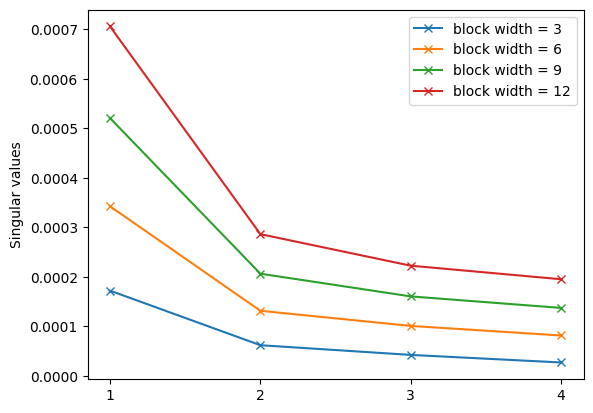
\includegraphics[width=0.7\textwidth]{singular_values.png}
        \caption{Mean singular values under different block widths.
        Since square blocks are used here, the block size is equal to
        the square of the width.}
        \label{FIG:SVAL}
    \end{figure}

    \hspace{1em} {\color{blue} Very good insight.
    This is connected to your major comment 4a)
    and we tried to attend them together.

    \hspace{1em} Yes, you are right that
    patch sizes should be width $\times$ height.
    We corrected this in the manuscript.

    % TODO: calculate nuclear norms of e.g. 2x2x4 and fullxfullx4 matrices
    \hspace{1em} The automatic estimation of the block size
    is described here (\url{https://mrtrix.readthedocs.io/en/dev/reference/commands/dwidenoise.html}),
    which suggests selecting "the smallest isotropic patch size
    that exceeds the number of DW images".

    \hspace{1em} We provide another notebook for explanations (\url{https://github.com/ZhengguoTan/demo_jets_diffusion_mri_7t/blob/main/demo_llr.ipynb}).
    As shown in \cref{FIG:SVAL}, larger block sizes lead to
    larger singular values, and thus also result in higher noise
    when the singular value thresholding value is kept consistent
    for different block sizes. Therefore, different block sizes require
    different singular value thresholds.
    }

    \item [11)] \textit{Sorry, I don't see that this has been attended.}

    \hspace{1em} {\color{blue} We added the row "slice thickness" in Table 1.}

    \item [12)] \textit{(New content) Reg. Eq. 6, L. "where the index k denotes the iteration" $\rightarrow$ this iteration was not in previous manuscript, unclear what it refers to.}

    \hspace{1em} {\color{blue} It refers to the iteration step
    of the iterative phase smoothing procedure.}

\end{enumerate}


% ========================================
%     Reviewer 249
% ========================================
\clearpage
\noindent \underline{\textbf{Reviewer \#249}}

\textit{I was pleased to see that
the Authors have put significant effort into this revision.
However some major concerns I had
regarding the description of the method and
its potential reproducibility still remain.}

\vspace{1em}

\noindent \textit{\# Major}

\vspace{1em}

\noindent \textit{\#\# Number of subjects}

\textit{I am happy that the Authors now state that they measured three subjects in the Methods section, but the presented data still only seem to show a single subject (e.g. in Fig. 9). Perhaps the Authors used a different subject for each separate experiment? Nevertheless, I would really like to see data from more than one subject for each experiment, even if this is put into an Appendix or Supplementary Information. Reproducing results in more than one subject is important to evaluate whether a method gives good results outside of a single (often "best") subject. If the main results do really each rely only on a single subject, I would strongly argue that each result should be reproduced in another subject before publication.}

    {\color{blue} Thank you for your comment.
    Because of the measurement time constraint,
    we used a different subject for each separate experiment.

    We recruited another subject to reproduce the results.
    Please refer to Supplementary Information for the results.}


\noindent \textit{\#\# Checkerboard artefact suppression (pg.~15)}

\begin{enumerate}
    \item \textit{I thank the Authors for providing the code that let me understand what the $T$ and $T^H$ operators are doing. However I now think that expressing the operation of $T$ and $T^H$ as matrix multiplication is very misleading. I would urge the Authors to rethink how they express this part. Probably it is e.g. better to write $T(x)$ instead of $Tx$, unless the authors explicitly define what the multiplication means in this non-standard operation.}

    \hspace{1em} {\color{blue} Thank you for looking into the code.
    We changed to $T(x)$ instead.}

    \item \textit{Further, I think $T^H$ needs to be better explained and justified. Where is it used? Are all the blocks reconstructed separately and then recombined for computational efficiency? Or is it just used when calculating the nuclear norm? It seems that $T^H$ is notation from the python package used by the Authors, but I think it is not very useful notation for those unfamiliar with that package. If I followed everything correctly, then what is really needed is an inverse of T (i.e. $T^{-1}$), but this is non-unique for overlapping blocks (one could have any combination of weights to recombine the overlapping elements as long as they sum to one). The Authors decided to take equal weights for each repeated elements, i.e. to take the mean, and I agree that this is probably the best choice to avoid checkerboard artefacts. However it would be much clearer (at least to me) if the authors expressed this in words, making clear that they take the mean of the overlapping elements, rather than in terms of an operator "$T^H$" and "multiplication" operations which are not defined by the Authors. The Authors could then point explicitly to the scripts they have written for details.}

    \hspace{1em} {\color{blue}
    First, the singular value thresholding (nuclear norm regularization)
    is calculated from the blocks, i.e., $T(x)$.
    Second, after the thresholding, $T^H$ is used to
    recombine the blocks to obtain the updated DW images.
    }

    \item \textit{If the operations really do need to be expressed in such detail, then it would perhaps be good to be explicit that the operation to get the "divisor" just gives the element-wise denominator for the mean.}

    \hspace{1em}{\color{blue} Thank you for the suggestion.
    We reworded the description.}

    \item \textit{The claim that this way of recombining blocks is efficient is not proven. I would suggest removing this claim.}

    \hspace{1em} {\color{blue} OK. We removed this statement.}

\end{enumerate}


\noindent \textit{\# Minor}

\vspace{1em}

\textit{My minor comments are mainly regarding the wording of some of the new text, which doesn't read as natural English to me. There are also some points which I didn't quite understand which the Authors could consider elaborating on further.}

{\color{blue} Sincerely thank you for your correction on the language.
We have corrected all of them and
highlighted the correction in the manuscript.
Therefore, no response was provided in the following comments
concerning language issues.}

\begin{enumerate}[resume]
    \item \textit{pg.~3: Techniques on the correction of... $\leftarrow$ Techniques for the correction of...}
    \item \textit{pg.~11: Different reconstruction methods, i.e., JETS, MUSE, and JULEP were compared. $\leftarrow$ Different reconstruction methods, specifically JETS, MUSE, and JULEP, were compared.}
    \item \textit{pg.~12: A possibility is to perform magnitude average... $\leftarrow$ One possibility is to perform magnitude averaging...}
    \item \textit{pg.~13: This can be incorporated to our formulation... $\leftarrow$ This can be incorporated into our formulation...}
    \item \textit{pg.~14: Please define the nuclear norm in Eq. (7). This would probably also help alleviate some of the problems with the description of the checkerboard artefact suppression mentioned above.}

    \hspace{1em} {\color{blue} Thank you. We defined the nuclear norm.}

    \item \textit{pg.~15: "This work employed blipped-CAIPI SMS (Setsompop et al., 2012), in which spatially separated slices are simultaneously excited and acquired. Therefore, 2D instead of 3D patches were used to construct the spatial-diffusion matrices." I don't understand how it follows from using multiband that 2D patches are used. Wouldn't this apply to all 2D sequences?}

    \hspace{1em} {\color{blue} Thank you for pointing this out.
    Here we reconstructed multiband slices jointly,
    but the multiband slices are spatially separated.
    This prohibits the use of 3D patches
    for the LLR regularization.
    We removed this part to avoid this confusion.}

    \item \textit{pg.~18: As show in Fig. 3... $\leftarrow$ As shown in Fig. 3...}
    \item \textit{pg.~18: ...the ripple-like phase artifact disapper after five iterations. $\leftarrow$ ...the ripple-like phase artifact disappears after five iterations.}
    \item \textit{Fig. 4: Please define what the arrows represent in the image caption.}

    \hspace{1em} {\color{blue} Done.}

    \item \textit{pg.~21: retrospecitvely $\leftarrow$ retrospectively}
    \item \textit{pg.~21: structural $\leftarrow$ Structural}
    \item \textit{Fig. 5: Please define what the arrows represent in the image caption.}

    \hspace{1em} {\color{blue} Done.}

    \item \textit{pg.~22: as pointed $\leftarrow$ as indicated}
    \item \textit{pg.~22: On the contrary $\leftarrow$ In contrast}
    \item \textit{pg.~22: First, we varied the regularization strength $\lambda$ from 0, to 0.08, and to 0.16. $\leftarrow$ First, we varied the regularization strength $\lambda$. We tested values of 0, 0.08, and 0.16.}
    \item \textit{pg.~22: "i.e., reduced noise" What does this mean? Perhaps you need to be more explicit?}

    \hspace{1em} {\color{blue} Done.}

    \item \textit{pg.~24: ...with the use of 5-shot acquisition. $\leftarrow$ ...with the use of a 5-shot acquisition.}
    \item \textit{pg.~24: When compared to the single-shot acquisition... $\leftarrow$ When compared to a single-shot acquisition}
    \item \textit{Fig. 8: The TRACE image at the bottom right seems to show aliasing near the bottom. Do you have an explanation for this?}

    \hspace{1em} {\color{blue} This may be caused by
    $B_1$ field inhmogeneity from the lower brain region. }

    \item \textit{pg.~29: ...MRI protocols in 7 T, e.g., 3-scan trace acquisition... $\leftarrow$ ...MRI protocols at 7 T, e.g., a 3-scan trace acquisition...}
    \item \textit{pg.~30: "The standard distortion correction method is known as TOPUP (Andersson et al., 2003), which acquires two scans with opposing phase-encoding directions to obtain the field inhomogeneity map and then performs conjugate phase reconstruction to correct for distortion." The B0 map does not need to come from TOPUP. Why not just collect a B0 map from multiecho data and incorporate it into the reconstruction? Often the multiecho data used to create SENSE maps for coil combination is used for this purpose.}

    \hspace{1em} {\color{blue} Thank you for the suggestion.
    We added this into Discussion.}

    \item \textit{pg.~30: "Beyond this SVT-based machine-learning reconstruction, one may seek to learn a q-space prior as the regularizer..." I don't understand what this sentence is trying to say. Is it a suggestion that machine learning could be used to learn a q-space prior?}

    \hspace{1em} {\color{blue} Yes, it is a suggestion that machine learning
    could be used to learn a $q$-space prior.}
\end{enumerate}


% ========================================
%     Reviewer 250
% ========================================
\clearpage
\noindent \underline{\textbf{Reviewer \#250}}

\textit{All points of my critique have been addressed adequately.}

\hspace{1em} {\color{blue} Thank you for your review.}

\end{document}